\section{Architecture}
MyMoodle is an extension of Moodle and can be seen as a package of plugins. 
The architecture does not specify how each plugins should be created but specify a general structuring of the parts of the system. 
The complete architecture can be seen in \figref{fig:architecture}.
\begin{figure}
	\centering
		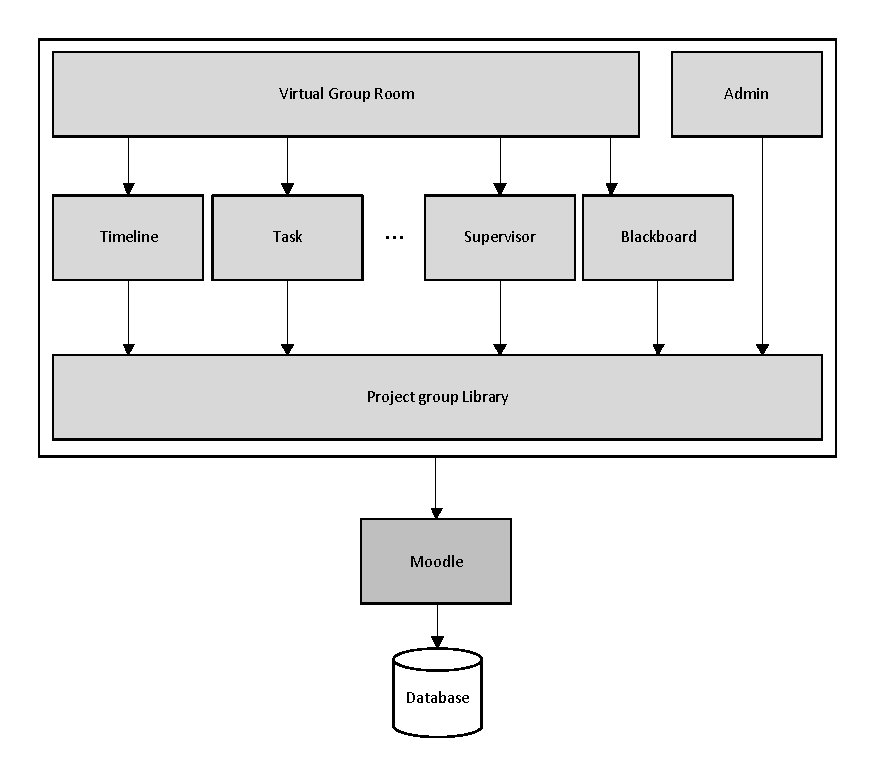
\includegraphics{images/architecture.pdf}
	\morscaption{The overall architecture of MyMoodle}
	\label{fig:architecture}
\end{figure}

The system consists of a total of five layers. 
The three uppermost is what we implement in this project, they have a common dependency of the Moodle platform. Layer four and five is respectiviely Moodle and the Database.
Our extension functions as a plugin of Moodle and use functions supplied by Moodle to function.

We will now explain the three uppermost layers:
\begin{enumerate}
	\item The upper most layer is the project group view and the administration tool. The project group view is used for presenting the project group room, described in \secref{sec:projectgroup}, and the administration tool, described in \secref{sec:projectgroupadministration}, is a tool used by administrative personal for creating, editing, and deleting project groups.
	\item Directly below the upper most layer is the ``middle'' layer which consist of the four parts: Timeline, Task, Supervisor, and Blackboard. These four parts are created by the other groups and are not explained further.
	\item Below the middle layer is the project group library which contain common functionality. This layer handles all communication between the parts in the middle layer.  
\end{enumerate}


There are two primary factors to be considered when planning an architecture. 
First, we are four sub-groups working together. 
This creates the need for a structured way of communicating between the different parts and it lets every sub-group know how their part is connected to the rest of the project. 
Second, the project should be passed on and with a solid and extendable architecture. 
Such an architecture increase the comprehensibility of the project and we deem that it will enhance the likelihood of a good pass on.
It is not possible to make a strict layered architecture due to the Moodle dependency and the administration tool which does not have use the intermediate layer, but depends directly on the project group library.

These considerations leet us to design the illustrated architecture.  

Exteding the architecture.













